% !TEX encoding = UTF-8
% !TEX TS-program = pdflatex
% !TEX root = ../tesi.tex

%**************************************************************
\chapter{Analisi dei requisiti}
\label{cap:analisi-requisiti}
%**************************************************************

\section{Confronto con gli stakeholders}
E' stato fatto un incontro iniziale con il proponente, ovvero l'azienda Sync Lab,
per definire con chiarezza i requisiti richiesti.
\\\\
Nell'incontro sono state prese in considerazione le REST API scritte col framework Spring 
già esistenti di cui doveva esserne fatta la migrazione nel framework NestJS.
E' emerso subito che la quantità di REST API da realizzare era troppo elevata per la
quantità di tempo a disposizione. 
\\\\
E' stato quindi necessario fare una valutazione di quali fossero i servizi fondamentali che
il servizio di REST API avrebbe dovuto esporre, per poter essere utilizzato senza che venissero
a mancare funzionalità fondamentali per l'utilizzo a livello base del sistema.
\\\\
Ho realizzato quindi un elenco di casi d'uso, in approvazione con la proponente, per avere più
chiari i requisiti del progetto.

\section{Entità}
Per rendere più chiaro il dominio del progetto ed eliminare eventuali ambiguità è stato necessario
documentare le entità di dominio, coinvolte nelle funzionalità fondamentali delle REST API, di cui si
è deciso effettuare la migrazione.
\\\\
Piazzola
\\
Modella il rettangolo bianco dipinto sull'asfalto che delimita la zona in cui l'automobile viene messa
in sosta. Ogni piazzola deve essere associata ad un parcheggio. Una piazzola può avere un solo sensore
di parcheggio.
\\
Ogni piazzola è caratterizzata da:
\begin{itemize}
    \item id: numero incrementale.
    \item latitudine: stringa.
    \item longitudine: stringa.
\end{itemize}
\leavevmode\newline
Parcheggio
\\
Modella l'insieme di piazzole.
\\
Ogni parcheggio è caratterizzato da:
\begin{itemize}
    \item id: numero incrementale.
    \item latitudine: stringa.
    \item longitudine: stringa.
\end{itemize}
\leavevmode\newline
Sensore
\\
Modella il sensore. Esistono due tipi di sensore:
\begin{itemize}
    \item ambientale: misurano la qualità dell'aria e altri parametri nel parcheggio e possono 
        coprire un'area di N piazzole.
        Sono gestiti da un'altro progetto di tirocinio, quindi non sono facenti parte di questo dominio di progetto.
    \item di parcheggio: sensore posizionato sotto l'auto nella piazzola, che rileva la presenza o meno
        del veicolo. Questo tipo di sensore può essere associato a una sola piazzola.
\end{itemize}
Ogni sensore può avere una sola azienda manutentrice a lui associata.
Ogni sensore è caratterizzato da:
\begin{itemize}
    \item id: numero incrementale.
    \item nome: stringa.
    \item batteria: stringa, indica la tensione della batteria in Volt.
    \item carica: stringa, indica il livello di carica della batteria (da 1 a 3).
    \item type: stringa, indica il tipo di sensore (ambientale o di parcheggio).
    \item attivo: booleano.
    \item ultimo sondaggio: data, indica l'ultima volta che è stato aggiornato lo stato del sensore.
    \item da riparare: booleano, indica se il sensore deve essere riparato.
    \item da caricare: booleano, indica se la batteria del sensore è scarica.
    \item in aggiornamento: booleano, indica se il sensore stà aggiornando il suo software.
\end{itemize}
\leavevmode\newline
Manutentore
\\
Modella l'azienda incaricata alla manutenzione dei sensori.
Ogni manutentore è caratterizzato da:
\begin{itemize}
    \item id: numero incrementale.
    \item nome: stringa, indica il nome del titolare dell'azienda.
    \item cognome: stringa, indica il cognome del titolare dell'azienda.
    \item azienda: stringa.
    \item telefono: stringa.
    \item email: stringa.
\end{itemize}
\leavevmode\newline
Misurazione sensore parcheggio.
\\
Modella la misurazione effettuata dal sensore di parcheggio. A differenza di un sensore ambientale, un sensore
di parcheggio non salva uno storico di misurazioni fatte ma viene inserita solo l'ultima misurazione effettuata,
sovrascrivendo la precedente.
Ogni misurazione di un sensore di parcheggio è caratterizzata da:
\begin{itemize}
    \item id: numero incrementale.
    \item indirizzo: stringa.
    \item latitudine: stringa.
    \item longitudine: stringa.
    \item valore: booleano, indica se il veicolo è presente o meno sopra al sensore.
    \item marca temporale: data, indica la data in cui è stata effettuata la misurazione.
\end{itemize}

\section{Casi d'uso}
Definite le entità di dominio si è proceduto con la creazione dei casi d'uso.
\\
Per maggior chiarezza i casi d'uso sono stati raggruppati per entità di dominio di appartenenza.
\\\\

% parcheggio
\begin{figure}[!h]
    \centering
    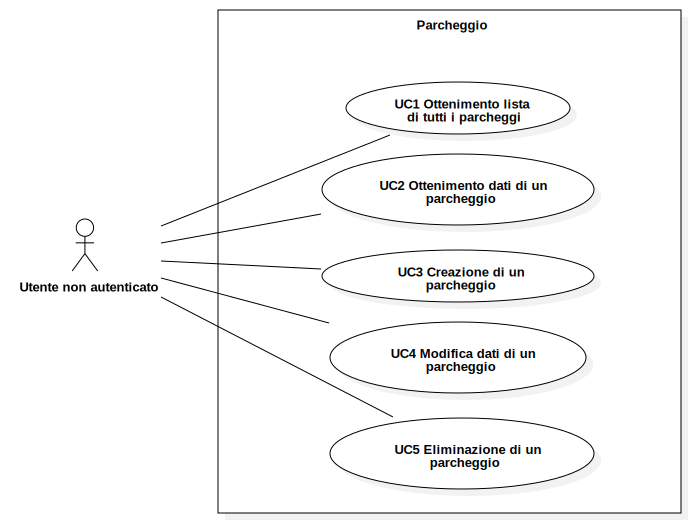
\includegraphics[height=9cm]{usecase/parking-area}
\end{figure}
UC1 - Ottenimento lista di tutti i parcheggi.
\\
Attori primari: utente non autenticato.
\\
Precondizioni: l'utente è in possesso degli strumenti per poter effettuare la richiesta al sistema.
\\
Post-condizioni: l'utente ha ottenuto una lista di tutti i parcheggi.
\\
Scenario principale:
\begin{enumerate}
    \item l'utente richiede la lista di tutti i parcheggi.
    \item l'utente ottiene una lista di tutti i parcheggi.
\end{enumerate}
\leavevmode\newline
UC2 - Ottenimento dati di un parcheggio.
\\
Attori primari: utente non autenticato.
\\
Precondizioni: l'utente è in possesso degli strumenti per poter effettuare la richiesta al sistema.
\\
Post-condizioni: l'utente ha ottenuto i dati di un parcheggio.
\\
Scenario principale:
\begin{enumerate}
    \item l'utente richiede i dati di un parcheggio.
    \item l'utente ottiene i dati di un parcheggio.
\end{enumerate}
\leavevmode\newline
UC3 - Creazione di un parcheggio.
\\
Attori primari: utente non autenticato.
\\
Precondizioni: l'utente è in possesso degli strumenti per poter effettuare la richiesta al sistema.
\\
Post-condizioni: l'utente ha creato un parcheggio.
\\
Scenario principale:
\begin{enumerate}
    \item l'utente richiede la creazione di un parcheggio.
    \item l'utente crea un parcheggio.
\end{enumerate}
\leavevmode\newline
UC4 - Modifica dati di un parcheggio.
\\
Attori primari: utente non autenticato.
\\
Precondizioni: l'utente è in possesso degli strumenti per poter effettuare la richiesta al sistema.
\\
Post-condizioni: l'utente ha modificato un parcheggio.
\\
Scenario principale:
\begin{enumerate}
    \item l'utente richiede la modifica di un parcheggio.
    \item l'utente modifica un parcheggio.
\end{enumerate}
\leavevmode\newline
UC5 - Eliminazione di un parcheggio.
\\
Attori primari: utente non autenticato.
\\
Precondizioni: l'utente è in possesso degli strumenti per poter effettuare la richiesta al sistema.
\\
Post-condizioni: l'utente ha eliminato un parcheggio.
\\
Scenario principale:
\begin{enumerate}
    \item l'utente richiede l'eliminazione di un parcheggio.
    \item l'utente elimina un parcheggio.
\end{enumerate}

% manutentore
\leavevmode\newline

\begin{figure}[!h]
    \centering
    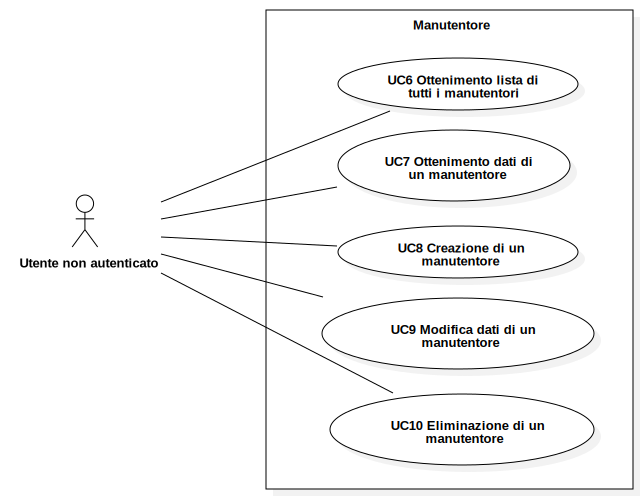
\includegraphics[height=9cm]{usecase/maintainer}
\end{figure}
UC6 - Ottenimento lista di tutti i manutentori.
\\
Attori primari: utente non autenticato.
\\
Precondizioni: l'utente è in possesso degli strumenti per poter effettuare la richiesta al sistema.
\\
Post-condizioni: l'utente ha ottenuto una lista di tutti i manutentori.
\\
Scenario principale:
\begin{enumerate}
    \item l'utente richiede la lista di tutti i manutentori.
    \item l'utente ottiene una lista di tutti i manutentori.
\end{enumerate}
\leavevmode\newline
UC7 - Ottenimento dati di un manutentore.
\\
Attori primari: utente non autenticato.
\\
Precondizioni: l'utente è in possesso degli strumenti per poter effettuare la richiesta al sistema.
\\
Post-condizioni: l'utente ha ottenuto i dati di un manutentore.
\\
Scenario principale:
\begin{enumerate}
    \item l'utente richiede i dati di un manutentore.
    \item l'utente ottiene i dati di un manutentore.
\end{enumerate}
\leavevmode\newline
UC8 - Creazione di un manutentore.
\\
Attori primari: utente non autenticato.
\\
Precondizioni: l'utente è in possesso degli strumenti per poter effettuare la richiesta al sistema.
\\
Post-condizioni: l'utente ha creato un manutentore.
\\
Scenario principale:
\begin{enumerate}
    \item l'utente richiede la creazione di un manutentore.
    \item l'utente crea un manutentore.
\end{enumerate}
\leavevmode\newline
UC9 - Modifica dati di un manutentore.
\\
Attori primari: utente non autenticato.
\\
Precondizioni: l'utente è in possesso degli strumenti per poter effettuare la richiesta al sistema.
\\
Post-condizioni: l'utente ha modificato un manutentore.
\\
Scenario principale:
\begin{enumerate}
    \item l'utente richiede la modifica di un manutentore.
    \item l'utente modifica un manutentore.
\end{enumerate}
\leavevmode\newline
UC10 - Eliminazione di un manutentore.
\\
Attori primari: utente non autenticato.
\\
Precondizioni: l'utente è in possesso degli strumenti per poter effettuare la richiesta al sistema.
\\
Post-condizioni: l'utente ha eliminato un manutentore.
\\
Scenario principale:
\begin{enumerate}
    \item l'utente richiede l'eliminazione di un manutentore.
    \item l'utente elimina un manutentore.
\end{enumerate}

% sensore
\leavevmode\newline
\begin{figure}[!h]
    \centering
    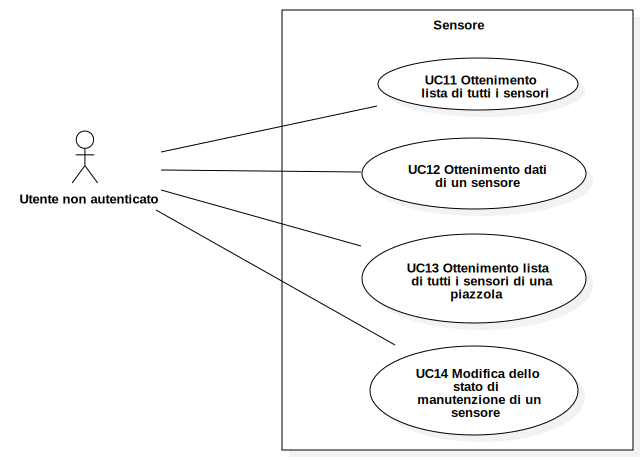
\includegraphics[height=9cm]{usecase/sensor}
\end{figure}
UC11 - Ottenimento lista di tutti i sensori.
\\
Attori primari: utente non autenticato.
\\
Precondizioni: l'utente è in possesso degli strumenti per poter effettuare la richiesta al sistema.
\\
Post-condizioni: l'utente ha ottenuto una lista di tutti i sensori.
\\
Scenario principale:
\begin{enumerate}
    \item l'utente richiede la lista di tutti i sensori.
    \item l'utente ottiene una lista di tutti i sensori.
\end{enumerate}
\leavevmode\newline
UC12 - Ottenimento dati di un sensore.
\\
Attori primari: utente non autenticato.
\\
Precondizioni: l'utente è in possesso degli strumenti per poter effettuare la richiesta al sistema.
\\
Post-condizioni: l'utente ha ottenuto i dati di un sensore.
\\
Scenario principale:
\begin{enumerate}
    \item l'utente richiede i dati di un sensore.
    \item l'utente ottiene i dati di un sensore.
\end{enumerate}
\leavevmode\newline
UC13 - Ottenimento lista di tutti i sensori di una piazzola.
\\
Attori primari: utente non autenticato.
\\
Precondizioni: l'utente è in possesso degli strumenti per poter effettuare la richiesta al sistema.
\\
Post-condizioni: l'utente ha ottenuto una lista di tutti i sensori di una piazzola.
\\
Scenario principale:
\begin{enumerate}
    \item l'utente richiede la lista di tutti i sensori di una piazzola.
    \item l'utente ottiene una lista di tutti i sensori di una piazzola.
\end{enumerate}
\leavevmode\newline
UC14 - Modifica dello stato di manutenzione di un sensore.
\\
Attori primari: utente non autenticato.
\\
Precondizioni: l'utente è in possesso degli strumenti per poter effettuare la richiesta al sistema.
\\
Post-condizioni: l'utente ha modificato lo stato di manutenzione di un sensore.
\\
Scenario principale:
\begin{enumerate}
    \item l'utente richiede la modifica dello stato di manutenzione di un sensore.
    \item l'utente modifica lo stato di manutenzione di un sensore.
\end{enumerate}

% piazzola
\leavevmode\newline
\begin{figure}[!h]
    \centering
    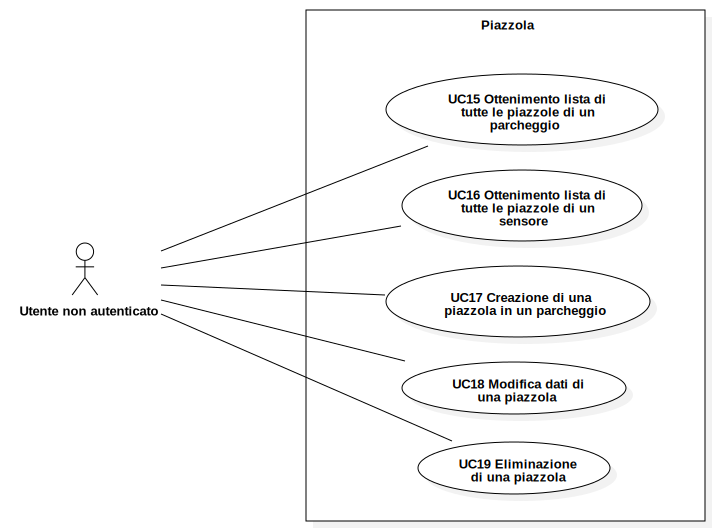
\includegraphics[height=9cm]{usecase/parking-spot}
\end{figure}
UC15 - Ottenimento lista di tutte le piazzole di un parcheggio.
\\
Attori primari: utente non autenticato.
\\
Precondizioni: l'utente è in possesso degli strumenti per poter effettuare la richiesta al sistema.
\\
Post-condizioni: l'utente ha ottenuto una lista di tutte le piazzole di un parcheggio.
\\
Scenario principale:
\begin{enumerate}
    \item l'utente richiede la lista di tutte le piazzole di un parcheggio.
    \item l'utente ottiene una lista di tutte le piazzole di un parcheggio.
\end{enumerate}
\leavevmode\newline
UC16 - Ottenimento lista di tutte le piazzole di un sensore.
\\
Attori primari: utente non autenticato.
\\
Precondizioni: l'utente è in possesso degli strumenti per poter effettuare la richiesta al sistema.
\\
Post-condizioni: l'utente ha ottenuto una lista di tutte le piazzole di un sensore.
\\
Scenario principale:
\begin{enumerate}
    \item l'utente richiede la lista di tutte le piazzole di un sensore.
    \item l'utente ottiene una lista di tutte le piazzole di un sensore.
\end{enumerate}
\leavevmode\newline
UC17 - Creazione di una piazzola in un parcheggio.
\\
Attori primari: utente non autenticato.
\\
Precondizioni: l'utente è in possesso degli strumenti per poter effettuare la richiesta al sistema.
\\
Post-condizioni: l'utente ha creato una piazzola in un parcheggio.
\\
Scenario principale:
\begin{enumerate}
    \item l'utente richiede la creazione di una piazzola in un parcheggio.
    \item l'utente crea una piazzola in un parcheggio.
\end{enumerate}
\leavevmode\newline
UC18 - Modifica dati di una piazzola.
\\
Attori primari: utente non autenticato.
\\
Precondizioni: l'utente è in possesso degli strumenti per poter effettuare la richiesta al sistema.
\\
Post-condizioni: l'utente ha modificato una piazzola.
\\
Scenario principale:
\begin{enumerate}
    \item l'utente richiede la modifica di una piazzola.
    \item l'utente modifica una piazzola.
\end{enumerate}
\leavevmode\newline
UC19 - Eliminazione di una piazzola.
\\
Attori primari: utente non autenticato.
\\
Precondizioni: l'utente è in possesso degli strumenti per poter effettuare la richiesta al sistema.
\\
Post-condizioni: l'utente ha eliminato una piazzola.
\\
Scenario principale:
\begin{enumerate}
    \item l'utente richiede l'eliminazione di una piazzola.
    \item l'utente elimina una piazzola.
\end{enumerate}

% misurazione
\leavevmode\newline
\begin{figure}[!h]
    \centering
    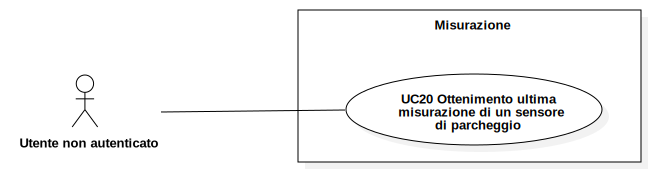
\includegraphics[height=9cm]{usecase/parking-sensor}
\end{figure}
UC20 - Ottenimento ultima misurazione di un sensore di parcheggio.
\\
Attori primari: utente non autenticato.
\\
Precondizioni: l'utente è in possesso degli strumenti per poter effettuare la richiesta al sistema.
\\
Post-condizioni: l'utente ha ottenuto l'ultima misurazione di un sensore di parcheggio.
\\
Scenario principale:
\begin{enumerate}
    \item l'utente richiede l'ultima misurazione di un sensore di parcheggio.
    \item l'utente ottiene l'ultima misurazione di un sensore di parcheggio.
\end{enumerate}

% TODO: inserire sotto casi d'uso specificando i campi da visualizzare / modificare
\section{Tracciamento dei requisiti}
Ogni requisito è identificato da un codice univoco nel seguente formato:
\begin{itemize}
    \item la prima lettera è sempre R, a indicare la parola requisito
    \item la seconda lettera indica il tipo di requisito:
    \begin{itemize}
        \item F per i requisiti funzionali
        \item Q per i requisiti qualitativi
        \item V per i requisiti di vincolo
    \end{itemize}
    \item un numero progressivo che identifica in modo univoco il requisito.
\end{itemize}
Per maggior chiarezza i requisiti sono stati raggruppati per entità di dominio di appartenenza.

% parcheggio
\leavevmode\newline
\begin{table}
    \begin{tabular}{|p{1cm}|p{6cm}|p{1.9cm}|p{1cm}|} 
    \hline
    Codice & Descrizione & Rilevanza &  Fonti \\ 
    \hline
    RF1 & L'utente non autenticato deve poter ottenere la lista di tutti i parcheggi. & Obbligatorio & UC1 \\ 
    \hline
    RF2 & L'utente non autenticato deve poter ottenere i dati di un parcheggio. & Obbligatorio & UC2 \\ 
    \hline
    RF3 & L'utente non autenticato deve poter creare un parcheggio. & Obbligatorio & UC3 \\ 
    \hline
    RF4 & L'utente non autenticato deve poter modificare i dati di un parcheggio. & Obbligatorio & UC4 \\
    \hline
    RF5 & L'utente non autenticato deve poter eliminare un parcheggio. & Obbligatorio & UC5 \\ 
    \hline
    \end{tabular}
\end{table}

% manutentore
\leavevmode\newline
\begin{table}
    \begin{tabular}{|p{1cm}|p{6cm}|p{1.9cm}|p{1cm}|} 
    \hline
    Codice & Descrizione & Rilevanza &  Fonti \\ 
    \hline
    RF6 & L'utente non autenticato deve poter ottenere la lista di tutti i manutentori. & Obbligatorio & UC6 \\ 
    \hline
    RF7 & L'utente non autenticato deve poter ottenere i dati di un manutentore. & Obbligatorio & UC7 \\ 
    \hline
    RF8 & L'utente non autenticato deve poter creare un manutentore. & Obbligatorio & UC8 \\ 
    \hline
    RF9 & L'utente non autenticato deve poter modificare i dati di un manutentore. & Obbligatorio & UC9 \\
    \hline
    RF10 & L'utente non autenticato deve poter eliminare un manutentore. & Obbligatorio & UC10 \\ 
    \hline
    \end{tabular}
\end{table}

% sensore
\leavevmode\newline
\begin{table}
    \begin{tabular}{|p{1cm}|p{6cm}|p{1.9cm}|p{1cm}|} 
    \hline
    Codice & Descrizione & Rilevanza &  Fonti \\ 
    \hline
    RF11 & L'utente non autenticato deve poter ottenere la lista di tutti i sensori. & Obbligatorio & UC11 \\ 
    \hline
    RF12 & L'utente non autenticato deve poter ottenere i dati di un sensori. & Obbligatorio & UC12 \\ 
    \hline
    RF13 & L'utente non autenticato deve poter ottenere la lista di tutti i sensori di una piazzola. & Obbligatorio & UC13 \\ 
    \hline
    RF14 & L'utente non autenticato deve poter modificare lo stato di manutenzione di un sensore. & Obbligatorio & UC14 \\ 
    \hline
    \end{tabular}
\end{table}

% piazzola
\leavevmode\newline
\begin{table}
    \begin{tabular}{|p{1cm}|p{6cm}|p{1.9cm}|p{1cm}|} 
    \hline
    Codice & Descrizione & Rilevanza &  Fonti \\ 
    \hline
    RF15 & L'utente non autenticato deve poter ottenere la lista di tutte le piazzole di un parcheggio. & Obbligatorio & UC15 \\ 
    \hline
    RF16 & L'utente non autenticato deve poter ottenere la lista di tutte le piazzole di un sensore. & Obbligatorio & UC16 \\ 
    \hline
    RF17 & L'utente non autenticato deve poter creare una piazzola in un parcheggio. & Obbligatorio & UC17 \\ 
    \hline
    RF18 & L'utente non autenticato deve poter modificare i dati di una piazzola. & Obbligatorio & UC18 \\
    \hline
    RF19 & L'utente non autenticato deve poter eliminare una piazzola. & Obbligatorio & UC19 \\
    \hline
    \end{tabular}
\end{table}

% misurazione
\leavevmode\newline
\begin{table}
    \begin{tabular}{|p{1cm}|p{6cm}|p{1.9cm}|p{1cm}|} 
    \hline
    Codice & Descrizione & Rilevanza &  Fonti \\ 
    \hline
    RF20 & L'utente non autenticato deve poter ottenere l'ultima misurazione di un sensore di parcheggio. & Obbligatorio & UC20 \\ 
    \hline
    \end{tabular}
\end{table}

% TODO: aggiungere requisiti facoltativi e desiderabili. Aggiungere requisiti qualitativi e di vincolo.